\chapter{Background}
\section{k-Anonymity}
\subsection{Motivation}
When an organisation releases a dataset containing personal information, they are responsible for ensuring the privacy of all participants. This is not an easy task and, as research has shown time and time again \cite{sweeney_uniqueness, rocher_estimating_reid, kanon_orig}, a lot of public datasets fall short of this privacy expectation. For example, as a first step, many organisations release datasets in which any explicit identifiers like names are removed. Nevertheless, in a lot of cases, the remaining information can be used to re-identify individuals by using unique combinations of fields in the dataset. 

For instance, in a paper published in 2000, Latanya Sweeney showed that 87\% of partipicants in the 1990 U.S. Census survey were uniquely identifiable by a combination of their zipcode, gender, and age \cite{sweeney_uniqueness}. As such, if we had the U.S. Census dataset, and knew someone's age, address, and gender, chances are we could recover the rest of their personal data, in what Sweeney coined a re-identification by linking. In 2002, she published a paper demonstrating this attack \cite{kanon_orig}.

Linking two datasets, Sweeney managed to re-identify the medical records of William Weld, the governor of Massachusetts at the time. The first dataset was a health insurance dataset, including information such as ethnicity, procedures undergone, medications given, etc..., for all state employees in Massachusetts. Weld, as governor, was in the dataset. This information was pseudonymised, thought safe, and sold to industry. The second dataset was the Registered Voters list for Cambridge, Massachusetts: a publicly available record of registered state voters in Cambridge (Weld's county of residence). This contained names, addresses, party affiliations, etc... The two sets had three fields in common: zipcode, birthdate, sex.

Because the Voter List included names, Sweeney found Weld's details. According to her, six people in the health insurance set had Weld's birthday, and only three of them were men. When you took the zipcode into account, he was the only one left. As such, Sweeney could guarantee that the medical record was his.

Although these examples are old, they're not outdated. In 2019, Luc Rocher, et al., published a paper showing that over 99\% of Americans could be reidentified using 15 demographic attributes \cite{rocher_estimating_reid}. Although 15 pieces of information seems less dangerous than Sweeney's combination of age, sex, and zipcode, we now collect considerably more data than twenty years ago, making this just as threatening.


These experiments exemplify the danger of releasing pseudonymised datasets under the assumption they're safe. In the same paper that uncovers the Massachusetts governor's medical history, Sweeney proposes a measure to thwart linking attacks: k-Anonymity. Informally, in a k-anonymous dataset, no individual's record is distinguishable from at least $k-1$ others. This ensures that even having auxiliary information on an individual, an attacker will always find at least $k$ records with this information, creating uncertain links. 

 For example, table ~\ref{fig:basic_example} (a) displays 4 records in a dataset containing zipcodes, ages, and incomes. If we were to know someone's age and zipcode, we could unequivocally infer their income. Table (b) shows the result after a 2-anonymization. In this case, we achieved it by generalizing our records, making zipcodes less specific when necessary and giving age ranges instead of exact numbers. Even if we had auxiliary information on someone, we couldn't be certain about their income. For example, we want to find someone's salary, and we know their zipcode, and age: 79203, and 27 respectively. In (a), their income is 64k. In (b), we now can't differentiate row 2 and 4 since the ages have been generalized and the target's salary could equally be 98k or 64k. In this example, we arbitrarily used 2 as our k-value but any k bigger than one will confer some measure of security, increasing with k.

%Basic Example tables
\begin{figure}
\centering
\subfigure[$D$]{
    \begin{tabular}{|l|l|l|l|}
        \hline
        ID & Zipcode & Age & Income \\
        \hline
        1  & 28488      & 33  & 52k    \\
        2  & 79203      & 24  & 98k    \\
        3  & 28473      & 39  & 36k    \\
        4  & 79203      & 27  & 64k    \\
        \hline
    \end{tabular}}
\subfigure[$D'$, 2-Anonymous]{
    \begin{tabular}{|l|l|l|l|}
        \hline
        ID & Zipcode & Age & Income \\
        \hline
        1  & 284** & 30's  & 52k    \\
        \rowcolor{gray!50}
        2  & 79203      & 20's  & 98k    \\
        3  & 284** & 30's  & 36k    \\
        \rowcolor{gray!50}
        4  & 79203      & 20's  & 64k    \\
        \hline
    \end{tabular}}
\caption{An example of a small dataset, and a 2-Anonymous version of it. The indistinguishable records are shaded in the same hue.}
\label{fig:basic_example}
\end{figure}

\subsection{Notations and Definitions}
First, we establish the notation and definitions we'll use through the report. These will be consistent with those used in Sweeney's paper originally presenting k-Anonymity \cite{kanon_orig}.


We will only be dealing with structured data. We define a tabular dataset, $D$, as a collection of rows representing records. A record $x_i$ is an ordered tuple of attributes, $x \in (A_1 \times \dots \times A_m)$ and, thus, $D=\{x_i\}_{i=1}^{|D|}$. We write $D[S]$ to mean taking the subset $S$ of columns in $D$.

Whilst every attribute is unique --- that is, no two columns contain the same information --- a tuple can reappear multiple times throughout the data. Nevertheless, every tuple belongs to one person, and no person has two tuples in the dataset.

Attributes can be categorized into three subsets:
\begin{itemize}
    \item \textit{direct identifiers}: attributes that, by themselves, can fully identify an individual in a dataset. These include, but are not limited to: names, phone numbers, or email addresses.
    \item \textit{quasi-identifiers} (QI): Attributes that contain personal information but aren't sufficient alone to uniquely identify a person in the dataset. These are pieces of information like ages, genders, or zipcodes.
    \item \textit{sensitive attributes}: private information that should not be linked back to individuals. For example, salaries, or medical records.
\end{itemize}

For example, a dataset $D[name, zipcode, gender, age, illness]$ containing a Hospital's patient information has one direct identifer: $name$. The set of quasi-identifiers is $QI=\{zipcode, gender, age\}$, and finally, the sensitive attribute is $illness$.

\begin{definition}{k-Anonymity} \\
A table $D$, with quasi-identifiers $QI_D$, is k-anonymous if and only if each tuple in $D[QI_D]$ appears at least k times in $D[QI_D]$.
\end{definition}

We have formalized what we described in the motivation. We want any combination of quasi-identifiers to be indistinguishable from $k-1$ others. An equivalent definition is that any auxiliary information an attacker could gather would point to at least $k$ records, making re-identification harder.

\begin{definition}{Equivalence Classes} \\
An equivalence class in $D$ with respect to the quasi-identifiers, $QI_D$, is the set of records having identical values for $D[QI_D]$ \cite{mondrian}.
\end{definition}

In other words, the equivalence classes are the sets of records that have indistinguishable quasi-identifiers. In k-anonymous datasets, these classes have a cardinality of at least $k$. As an example, Table (a) in Figure ~\ref{fig:basic_example} has two equivalence classes: $\{1,3\}$ and $\{2,4\}$.

\subsection{Generalization and Suppression}
In this section, we formalize the theory of generalization, hinted at in the motivation.

At a first glance, k-anonymity could be achieved by removing all records that don't have equivalent classes of sufficient size. However, this can result in a lot of lost information. For that reason, most algorithms work with some form of generalization: instead of removing rows, tuples are replaced with more generic versions of them, allowing them to fit in broader equivalence classes \cite{kanon_algos}\cite{mondrian}. For example, in Figure ~\ref{fig:basic_example}, we achieve this by stripping the rightmost digits of a zipcode, thus referencing a larger geographical area, or by giving a range of ages instead of specific values. To formalize the way we approach attributes, and to facilitate the description of how to generalize them, we need to define a \textit{domain}:

\begin{definition}{Domain} \\
A domain is the set of values an attribute can take \cite{kanon_algos}. Domains can be continuous (e.g., a salary $\in \mathbb{R}$) or discrete (e.g., zipcodes $\subset \mathbb{Z}$ or categorical attributes like nationality: \{English, American, ...\}). The \textit{ground} domain of an attribute is the domain that hasn't been generalized at all. For instance, the ground domain of zipcodes, $Z_0$, is a string of any five digits. Domains can be generalized to make attributes less informative; say, $Z_1$ where $93772 \mapsto 9377*$. These build to become less and less specific $(Z_0, Z_1, Z_2...)$.
\end{definition}

We can see that for any domain, we need a function mapping every level of generalization to the next one -- i.e., for an attribute $A$, we need functions $\phi_i$ such that each is a generalization from a domain $A_i$ to the next generalized domain $A_{i+1}$. This will allow us to move from specific values to increasingly generalized ones. This is concept is formally respresented by \textit{Value Generalization Hierarchies}, and \textit{Domain Generalization Hierarchies}:

\begin{definition}{Value and Domain Generalization Hierarchy (VGH, DGH)}\\
For a quasi-identifier $A$, with a ground domain $A_0$, we need a set of surjective functions:

$$\phi_{A_i}: A_{i} \to A_{i+1}, \mbox{ for } i=0,...,n-1 \mbox{, such that } |A_n|=1$$ 

These functions reduce the size of the domain at every level, generalizing the values in them. This is called a Value Generalization Hierarchy ($VGH_A$).  

Additionally, we define the set of domains $\{A_i| i = 0,...,n\}$ as the Domain Generalization Hierarchy ($DGH_A$).
\end{definition}

The definition of a $VGH$ implies that every attribute is eventually generalized to a null value since $A_n$, the top level, only contains one element and everything must thus map to it. For example, going back to our zipcode example, if we assume every further generalization strips off the rightmost digit, we see that the highest level of generalization, $\phi_4$, maps any $x**** \mapsto *****$ and leaves us with a suppressed value; it divulges no information.

Intuitively, Value Generalization Hierarchies can be thought of as the generalization trees that will be used for values, Domain Generalization Hierarchies represent the actual values present at every level.

For example, Figure ~\ref{fig:tree_zip} displays the $DGH$ on $Z$, the zipcode attribute, if our dataset had a ground domain $Z_0 = \{x \in \mathbb{N} | 19300 \leq x < 19400 \}$. Notice that we go from $Z_2$ to total suppression. This is because $Z_2$ is singleton, implying further generalizations are pointless since we'll still have only one class of zipcodes.

%VHG Zip
\begin{figure}
\centering
\subfigure[$DGH_Z$]{
    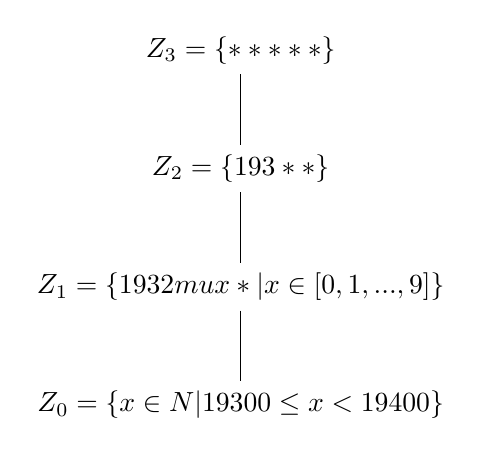
\begin{tikzpicture}[sibling distance=6em,
    level 2/.style={sibling distance=10em},
    level 3/.style={sibling distance=5em}]]
    \node {$Z_3 = \{*****\}$}
    child {node {$Z_2 = \{193**\}$}
    child {node {$Z_1 = \{193 \mspace{2mu}x* | x \in [0,1,...,9]    \}$}
    child {node {$Z_0 = \{x \in \mathbb{N} | 19300 \leq x < 19400 \}$}
    }}};
    \end{tikzpicture}}
\subfigure[$VGH_{Z}$]{
    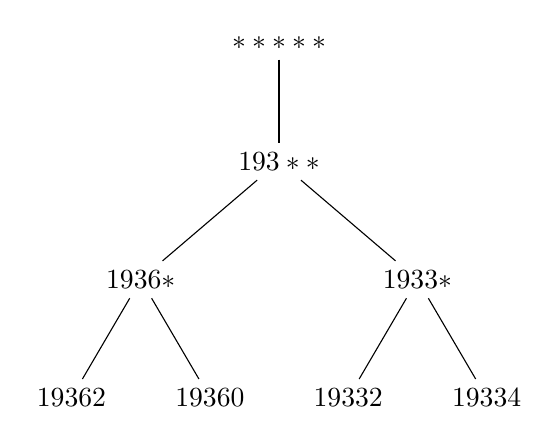
\begin{tikzpicture}[sibling distance=6em,
    level 2/.style={sibling distance=10em},
    level 3/.style={sibling distance=5em}]]
    \node {$*****$}
    child { node {$193**$} 
        child { node {$1936*$}
            child { node {$19362$}}
            child { node {$19360$}}
        }
        child { node {$1933*$}
            child { node {$19332$}}
            child { node {$19334$}}
        }
    };
    \end{tikzpicture}}
\caption{A DGH, and VGH for an example zipcode quasi-identifier}
\label{fig:tree_zip}
\end{figure}

It's important to point out that we can also create $VGH$s for categorical attributes. An example is provided in Figure ~\ref{fig:tree_ed}, with a level of education attribute $A_{ed}$ where we generalize the level of study to whether any further studies were undertaken after High School. The choice of the mapping is up to us, the data curators. For instance, we could also have decided that the difference between a Masters degree and a PhD was significant enough to warrant a third group, "Further Studies+" at the first level of generalization. This would give an alternative, but equally valid, VGH.

%VGH education
\begin{figure}
\centering
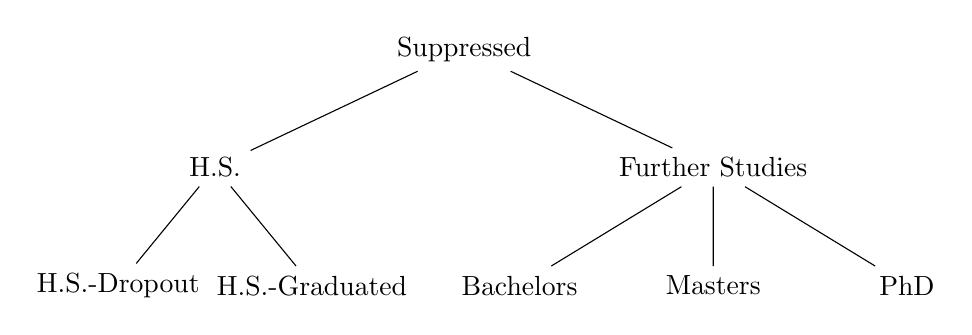
\begin{tikzpicture}[sibling distance=6em,
level 1/.style={sibling distance=18em},
level 2/.style={sibling distance=7em}]]
\node {Suppressed}
child { node {H.S.} 
    child { node {H.S.-Dropout}}
    child { node {H.S.-Graduated}}
}
child { node {Further Studies} 
    child { node {Bachelors}}
    child { node {Masters}}
    child { node {PhD}}
};
\end{tikzpicture}
\caption{An example VGH for a level of education attribute}
\label{fig:tree_ed}
\end{figure}

Finally, we introduce notation to define order in how generalized a dataset is:

\begin{definition}{Ordering Generalizations} \\ 
For a dataset $D$, and $D'$, a generalization of $D$. We introduce the notation $D \leq D'$ as a partial ordering meaning that $D'$ is a generalization of $D$. 
\end{definition}


\subsection{Existing Algorithms}

Because every $k$-anonymization involves generalizations and suppressions, although information does not change, it is coarsened, losing detail. We therefore aim to find algorithms that minimize how coarse the output is. However, we also have to take into account that there is a tradeoff with complexity -- if an algorithm takes too much time, then its applicability decreases. 

Before we can describe the algorithms, we introduce different generalization techniques that exist. The first is \textit{global single-dimensional generalization}:

\begin{definition}{Global Single-Dimensional Generalization} \\ 
On a table $D$ of size $n$, for an attribute $ A \in QI_D$, a global single-dimensional generalization on $A$ is the application of the functions defined for $VGH_A$ on the entire attribute column. We had defined a function at cell level so we extend the definition for an entire column with $n$ entries:  $\phi_{A_i}^{(n)}$, with $\phi_{A_i}^{(n)}: A_i^{(n)} \to A_{i+1}^{(n)}$, where $A_{i+1}$ is the next generalized domain. \cite{mondrian}

For example, reusing our defined VGH in Figure \ref{fig:tree_ed}, if our education column was as followed: $C_{ed_0} = ($Bachelors, PhD, PhD, H.S.-Graduated$)$, then a Global Single-Dimensional Generalization returns $C_{ed_1}$:
\[C_{ed_1} = (\text{Further Studies, Further Studies, Further Studies, H.S.})\]
We can generalize $C_{ed_1}$ one step further, to suppression:
\[C_{ed_2} = (\text{Suppressed, Suppressed,Suppressed,Suppressed})\]

This type of generalization is single-dimensional, meaning it has a specific mapping for every quasi-identifier defined in the VGH, and global because it generalizes an entire attribute column at once.
\end{definition}

To allow for more flexibility, we can generalize on combinations of a table's quasi-identifiers:
\begin{definition}{Global Multidimensional Generalization} \\ 
Let $D$ be a dataset with quasi-identifiers $(A_1,...,A_n)$. Instead of having a function per quasi-identifier, we define a single function $\phi: A_1 \times ... \times A_n \to A_1' \times ... \times A_n'$ that generalizes by the record. The only requirement is that $A_i'$ is equally as general or moreso than $A_i$. This allows for more flexible generalizations as we don't need to ensure every column is $k$-anonymous independently.

For example, take Figure \ref{fig:multi_vs_singledim_example}. $D''$ is a $2$-anonymous version of $D$ done using a global multidimensional generalization. We see that its Zipcode column isn't generalized to the same extent for every value, leaving us with more detail than in $D'$, anonymized by applying single-dimensional generalizations.
\end{definition}

%multi vs. single dimensional Example tables
\begin{figure}
\centering
\subfigure[$D$, A dataset]{
    \begin{tabular}{|l|l|l|}
        \hline
        Zipcode & Age & Income \\
        \hline
        28498 & 30's  & 52k    \\
        79203 & 20's  & 98k    \\
        28473 & 30's  & 36k    \\
        79203 & 20's  & 64k    \\
        \hline
    \end{tabular}}
\subfigure[$D'$, Global Single-Dimensional Generalization]{
    \begin{tabular}{|l|l|l|}
        \hline
        Zipcode & Age & Income \\
        \hline
        284** & 30's  & 52k    \\
        284** & 30's  & 36k    \\
        \rowcolor{gray!50}
        792**      & 20's  & 98k    \\
        \rowcolor{gray!50}
        792**      & 20's  & 64k    \\
        \hline
    \end{tabular}}
\subfigure[$D''$, Global Multidimensional Generalization]{
    \begin{tabular}{|l|l|l|}
        \hline
        Zipcode & Age & Income \\
        \hline
        284** & 30's  & 52k    \\
        284** & 30's  & 36k    \\
        \rowcolor{gray!50}
        79203      & 20's  & 98k    \\
        \rowcolor{gray!50}
        79203      & 20's  & 64k    \\
        \hline
    \end{tabular}}
\caption{An example demonstrating the difference between a single-dimensional and a multidimensional global generalization on table $D$. Equivalence classes are shaded in the same hue. We notice that we can preserve more detail on the zipcode attribute by generalizing Multidimensionally.}
\label{fig:multi_vs_singledim_example}
\end{figure}

The alternative approach is to attempt generalization locally. For example, we can partition our dataset into a \textit{multi-dimensional region}:

\begin{definition}{multi-dimensional region} \\
On a table $D$, with quasi-identifiers $A_1, A_2, ..., A_m$. Assuming a total order on these attributes, we can partition the dataset into regions defined by a pair of tuples $(l_1, ..., l_m),(u_1,...,u_m) \in A_1\times A_2\times ... \times A_m$ such that $\forall i, l_i \leq u_i$ \cite{mondrian}. Intuitively, this equates to partitioning $D$ into $m$-dimensional rectangular boxes that cover the state-space. 

The generalizing function $\phi$ maps each tuple $(x_1, ..., x_m) \in A_1\times A_2\times ... \times A_m$ to a summary statistic of the region it contains. These summary statistics can take many shapes, the simplest one being a range of values present in the region. 
\end{definition}

From the many algorithms that have been proposed, (\cite{ola_algo}\cite{mondrian}\cite{incognito}\cite{kanon_algos}), we'll describe a few of particular interest: MinGen, Datafly, and Mondrian. Datafly is the first algorithm proposed by Sweeney \cite{sweeney_datafly}. She later introduced MinGen, the first algorithm optimised for a utility metric,  and, finally, Mondrian-- an efficient local generalization algorithm \cite{mondrian}. 

\subsubsection{DataFly: Greedy Single-Dimensional Generalization}
In 1997, before formalizing the concept of k-anonymization, Sweeney developed a practical anonymization algorithm called Datafly \cite{sweeney_datafly}. Datafly works by greedily generalizing the quasi-identifier with the largest domain, using a Global Single-Dimensional approach. It does so iteratively, until the table is k-anonymous, or close enough to warrant suppressing a few records. 

For a dataset $D$, the algorithm revolves around a frequency table of the tuples in $D[QI_D]$. Whilst more than k records in the frequency table are not anonymous, Datafly will generalize an attribute, and update the frequency table accordingly. At the end, the small amount of leftover non-anonymous records are removed, and the dataset is rebuilt from the frequency table -- i.e., a tuple with a certain count is inserted that many times in a new table. The following is outlined in Algorithm \ref{datafly}. In this pseudo-algorithm, \textit{generalize} means to globally and single-dimensionally generalize the attribute with the generalization function from the VGH with the appropriate depth.
%Datafly
\begin{algorithm}
\caption{Datafly: a practical k-anonymization}
\label{datafly}
\textbf{Input:} Table $D$; a defined $DGH$ for every $QI$; a fixed k. \\
\textbf{Output:} $D'$, a k-anonymous generalization of $D$
\begin{algorithmic} % enter the algorithmic environment
    \Ensure $|T| > k$
    
    \State freq $\leftarrow \{\forall t \in T[QI_T]: (t, count(t, T[QI_T]))\}$     
    \While{more than k tuples in freq are not k-anonymous}
        \State $A_j \leftarrow \max_{A \in QI}(|\{\mbox{freq}[A]\}|)$ 
        \State freq$[A_j] \leftarrow generalize($freq$[A_j])$
    \EndWhile
    \State freq $\leftarrow$ suppress tuples occuring less than k times
    \State $GT \leftarrow rebuild($freq$)$ \\
    \Return $GT$
    
\end{algorithmic}
\end{algorithm}

This algorithm is fast but may distort data more than necessary due to the fact it makes ``crude decision'' in generalizing entire columns at once. Furthermore, it heavily penalizes attributes with a wide range of different values, leading to unecessary generalizations. For example, if we had a table $D(ZIP, gender)$, our domain $ZIP_4$, containing things of the form x**** would contain up to 10 different elements whereas $gender_0$ would have two at most. This means that before Datafly even considers generalizing gender, it would fully suppress the zipcode.


\subsubsection{MinGen: Minimal Generalization}
\label{mingen}
As mentioned above, we are looking to keep our data as integral as possible and Datafly doesn't always satisfy that requirement. To rectify that, Sweeney proposed MinGen in 2002\cite{kanon_algos}. MinGen is naive, and "makes no claim to be efficient" but guarantees k-anonymity with the minimal amount of generalization over the quasi-identifiers using global single-dimensional generalizations. 

We define minimal generalization:

\begin{definition}{k-Minimal Generalization} \\
Let $D_l(A_1,...,A_n)$ and $D_m(A_1,...,A_n)$ be two tables such that $D_l[QI] \leq D_m[QI]$ where $QI$ is the set of quasi-identifiers associated with the tables. $D_m$ is said to be a k-minimal generalization of $D$ over $QI$ if and only if:
\begin{itemize}
    \item $D_m$ satisfies the k-anonymity property
    \item $\forall$ k-anonymous $D_z$ satisfying $D_l \leq D_z$ and $D_z \leq D_m$ then $D_z = D_m$. 
\end{itemize}
\end{definition}

In other words, this definition helps us find the first generalized table that is k-anonymous. Nevertheless, every table could have multiple k-minimally generalized tables, and they wouldn't all be as useful. For example, Table \ref{fig:kminimal_gen_tables} depicts two different k-minimal generalizations of a Table $D$: we could either generalize zipcode by removing the last three digits, or by generaling both zipcode and age once. They're both 2-anonymous, and any $G$ with $G \leq D'$ or $G \leq D''$ wouldn't be, implying 2-minimal generalization. The question now becomes, which should we use?

%Min generalization example
\begin{figure}
    \centering
    \subfigure[$D$]{
    \begin{tabular}{|c|c|}
    \hline
    Zipcode & Age \\
    \hline
    97385 & 21 \\
    97412 & 21 \\
    97492 & 36 \\
    97365 & 36 \\
    \hline
    \end{tabular}}
    \subfigure[$D'$]{
    \begin{tabular}{|c|c|}
    \hline
    Zipcode & Age \\
    \hline
    973** & [20-40] \\
    974** & [20-40] \\
    974** & [20-40] \\
    973** & [20-40] \\
    \hline
    \end{tabular}}
    \subfigure[$D''$]{
    \begin{tabular}{|c|c|}
    \hline
    Zipcode & Age \\
    \hline
    97*** & 21 \\
    97*** & 21 \\
    97*** & 36 \\
    97*** & 36 \\
    \hline
    \end{tabular}}
    \caption{Different $k$-minimal generalizations for a table $D$. $D'$ generalizes twice on zipcode and once on age. Revert any of these generalizations and our table is no longer $2$-anonymous, implying it is a minimal generalization. Instead, $D''$ generalizes further on the zipcode but leaves age untouched. It is also a $2$-minimal generalization.}
    \label{fig:kminimal_gen_tables}
\end{figure}

To solve that, Sweeney, et al., define a preference criteria in the form of the precision metric (defined in \nameref{metrics_prec}) which captures the amount of information lost and we define minimal distortion:

\begin{definition}{k-Minimal Distortion} \\
Let $D_l(A_1,...,A_n)$ and $D_m(A_1,...,A_n)$ be two tables such that $D_l[QI] \leq D_m[QI]$ where $QI$ is the set of quasi-identifiers associated with the tables. $D_m$ is said to be a k-minimal distortion of $D$ over $QI$ if and only if:
\begin{itemize}
    \item $D_m$ satisfies the k-anonymity property
    \item $\forall$ k-anonymous $D_z$ satisfying $Prec(D_l) \geq Prec(D_z)$ and $Prec(D_z) \geq Prec(D_m)$ then $D_z = D_m$. 
\end{itemize}
\end{definition}

Furthermore, Sweeney states as a Theorem: 
\begin{thm}\cite{kanon_algos}
    Given datasets $D_l$ and $D_m$ such that $D_l \leq D_m$, and $D_m$ satisfying k-anonymity. $D_m$ is a k-minimal distortion of $D_l$ $\implies$ $D_m$ is a k-minimal generalization of $D_l$.
\end{thm}


Puting these together, we can now limit our search to the the minimal distortion, and an algorithm starts to form. Given a Table $D(A_1,...,A_n)$ with $QI = \{A_i,...,A_j\} \subseteq (A_1,...,A_n)$, a k, and a $DGH_i$ for every $i$ in $QI$, the first step is verifying if $D$ is already k-anonymous. In that case, we're done since it will be minimally generalized. If it isn't, we store every possible generalization of $D$ over $QI$. We then filter out any that don't satisfy the k-anonymity condition. From the leftover anonymous tables, we need to find the one that is minimally distorted, which we do by calculating the distortion of every generalization. If we still get multiple generalizations with the same Precision, then we let the user pick which generalization they want to use because, depending on their use for the data, they might prefer generalizing certain attributes over others. Another strategy to deal with user preferences is to assign weights to the attributes, giving them more or less importance. we outline the MinGen algorithm in Algorithm \ref{mingen_kmin_gen}. In this version, we assume all attributes to have equal importance.

%MinGen 
\begin{algorithm}
\caption{MinGen: k-minimally generalized}
\label{mingen_kmin_gen}
\textbf{Input:} Table $D$; a defined $DGH$ for every $QI$; a fixed k; a \textbf{preferred} function defined by user to choose one generalization amongst multiple solutions.\\
\textbf{Output:} MGT, a k-minimal distortion of $D$, chosen according to preference
\begin{algorithmic} % enter the algorithmic environment
    \Ensure $|D| > k$
    \If {anonymous$(D)$}
        \State MGT $\leftarrow$ $D$
    \Else
        \State allgen $\leftarrow$ $\{D_i: D_i$ is a generalization of $D\}$
        \State anon $\leftarrow$ $\{D_i: D_i \in$ allgen $\And$ $D_i$ is anonymous $\}$
        \State MGT $\leftarrow$ $\{D_i: D_i \in$ anon $\And \not\exists D_z \in$ anon s.t. $Prec(D_z) \geq Prec(D_i)\}$
        \State MGT $\leftarrow$ \textbf{preferred}(MGT)
    \EndIf \\
    \Return MGT
    
    
\end{algorithmic}
\end{algorithm}

In 2004, Meyerson and Williams proved that finding an optimal k-anonymous generalization is an NP-hard problem \cite{meyerson2004complexity}. This confirms Sweeney's claim of inefficiency, and makes it an untractable algorithm to use on any meaningful dataset. As such, although this algorithm produces optimal results for global single-dimensional generalizations, we'll primarily rely on the other algorithms to get tractable problems.


\subsubsection{Mondrian: Greedy Region Partitioning}
In 2006, LeFevre, DeWitt, and Ramakrishnan, et al. came up with a greedy algorithm for multidimensional generalization using a partition based model \cite{mondrian}. This is different from Sweeney's single dimension generalization algorithms, MinGen and Datafly, in the sense that it partitions the dataset in heuristically similar subsets of size at least k, and then generalizes them using a Multidimensional Region approach. This satisfies the k-anonymity property since every subset contains at least k indistinguishable generalized records. It also allows more flexibility as we're not generalizing at the column level, but rather at the partition level, which means we can avoid generalizing subsets that are already anonymous, distorting data for no reason. 

Visualizing our data as a $|QI|$-dimensional space, we heuristically pick a dimension (i.e., an attribute), and create a cut at the median value. This cut separates our table into two subsets on which we recursively keep partitioning. We do this until we can't find a cut that would give us two regions with at least k elements in them. Once we've got our regions, we generalize them to the same tuple. A good way to do this is through a summary statistic-- a function that statistically summarizes every dimension of the region. For example, these can be ranges, or averages.

Different heuristics exist to pick attributes to cut on. Usually, the attribute with the widest normalized range of values but we have flexibility on that.

In Algorithm \ref{mondrian_pseudocode}, we outline the Mondrian algorithm, assuming every attribute has been ordered correctly. `choose\_dim' gives the user a choice on the heuristic to select the attribute to cut on and `summary\_statistic' explains how to generalize the different dimensions.

%Mondrian
\algdef{SE}[FUNCTION]{Function}{EndFunction}%
   [2]{\algorithmicfunction\ \textproc{#1}\ifthenelse{\equal{#2}{}}{}{(#2)}}%
   {\algorithmicend\ \algorithmicfunction}%
\begin{algorithm}
\caption{Mondrian: Multi-Dimensional Greedy Partitioning k-anonymization}
\label{mondrian_pseudocode}
\textbf{Input:} Table $D$; a fixed k; choose\_dim function; choose summary\_statistic function \\
\textbf{Output:} $D'$, a k-anonymous generalization of $D$
\begin{algorithmic} % enter the algorithmic environment
    \Ensure $|D| > k$
    \Function{Partition}{region}
        \If{no allowable cut on region}
            \Return summary\_statistic(region)
        \Else
            \State $A_j \leftarrow$ choose\_dim(region)
            \State $med \leftarrow$ median(region[$A_j$])
            \State $lhs \leftarrow \{t \in \mbox{region}: t[A_j] \leq med\}$
            \State $rhs \leftarrow \{t \in \mbox{region}: t[A_j] > med\}$
        \EndIf \\
        \Return $\textproc{partition}(lhs) \cup \textproc{partition}(rhs)$
    \EndFunction
\end{algorithmic}
\end{algorithm}

Figure \ref{fig:mondrian_ex} shows an example of how a Mondrian partition would choose cuts on a set containing zipcodes and education levels: subfigure(a). The largest domain is education, and as such, Mondrian cuts the domain as equally as possible (b). The right and left partitioned are subsequently divided independently (c, and d). This repeats until no allowable cut exists because the subsets are too small. We now anonymize every partition. Notice that we'll anonymize different partitions differently, allowing for more fine-grained generalization:

\begin{multline}
    \{(\mbox{H.S Dropout}, 34986), (\mbox{H.S Dropout}, 34917)\}
    \mapsto \\
    \{(\mbox{H.S. Dropout}, 34***),(\mbox{H.S. Dropout},
    34***) \}
    \label{mondrian_gen1}    
\end{multline}
\begin{equation}
     \{(\mbox{Masters}, 34986), (\mbox{PhD}, 34986)\} \mapsto \{(\mbox{Further Studies}, 34986), (\mbox{Further Studies}, 34986)\}
     \label{mondrian_gen2}
\end{equation}

%Mondrian cut example
\begin{figure}
    \centering
    \subfigure[Initial representation]{
        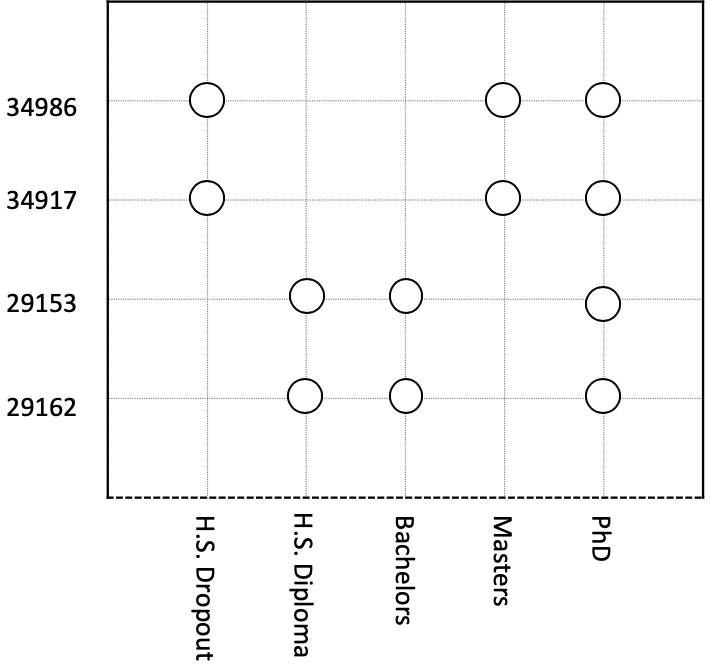
\includegraphics[scale=0.5]{background/fig/mondrian0.png}
    }
    \subfigure[First cut]{
        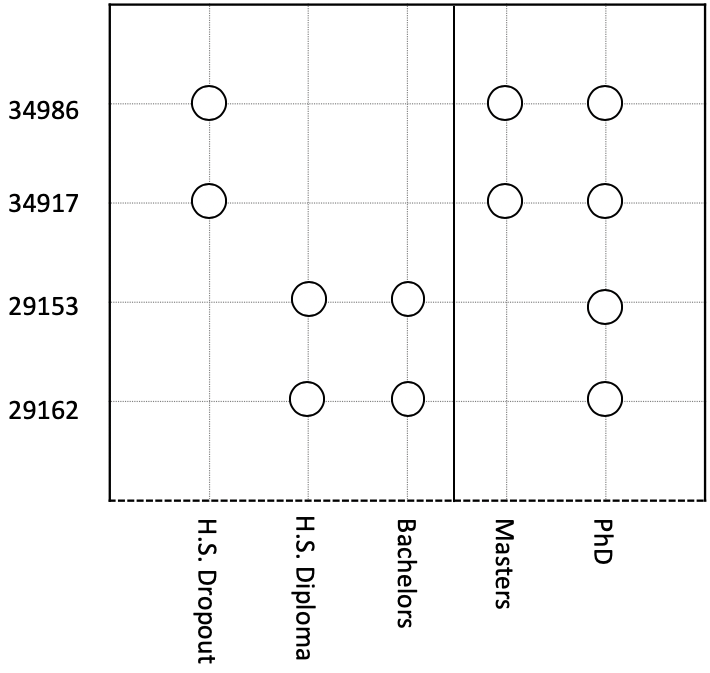
\includegraphics[scale=0.5]{background/fig/mondrian1.png}
    }
    \subfigure[Second cuts]{
        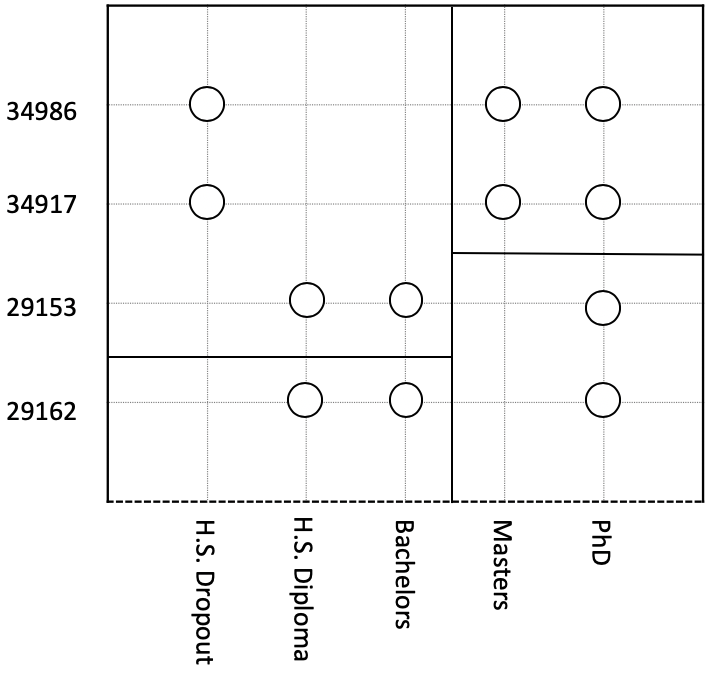
\includegraphics[scale=0.5]{background/fig/mondrian2.png}
    }
    \subfigure[Third and final cuts]{
        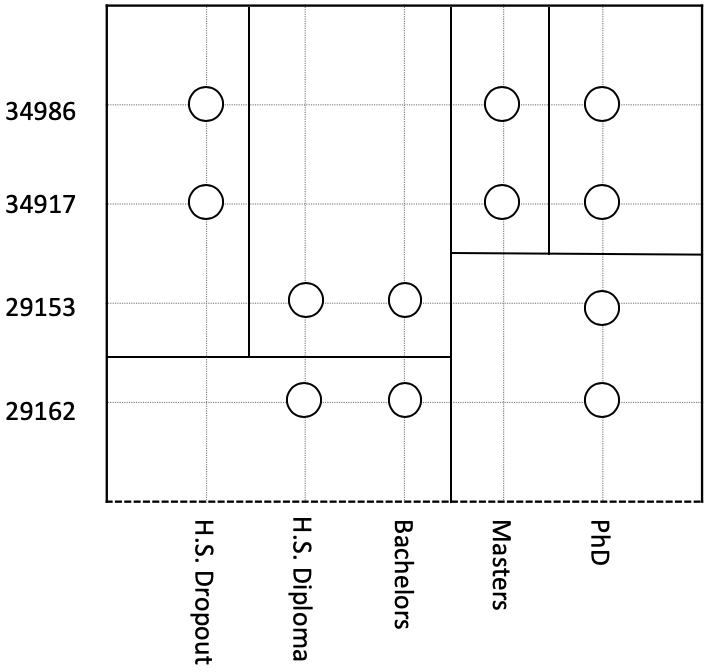
\includegraphics[scale=0.5]{background/fig/mondrian3.png}
    }
    \caption{A Figure representing the four steps in an example Mondrian $2$-anonymizing dataset containing two quasi-identifier, education level and zipcode. (a) is a 2D visualization of the two attributes. In (b), we show the first cut, separating the datapoints in two, along the axis with the largest normalized range of values. In (c), we see two additional cuts on the subsets, this time along the zipcode axis. Finally, the third cuts in (d) reveal the final regions for this Mondrian algorithm. We cannot go further otherwise we break the $k$ constraint.}
    \label{fig:mondrian_ex}
\end{figure}

Additionally, Mondrian has the additional flexibility of making DGHs for every quasi-identifier optional. Every region is bounded, and these can serve as generalization. Any numerical attribute has a clear lower and upper bound. In the absence of a DGH for the example in Figure \ref{fig:mondrian_ex}, the generalization examples we saw in \eqref{mondrian_gen1} and \eqref{mondrian_gen2} could have been as shown in \eqref{mondrian_no_dgh1} and \eqref{mondrian_no_dgh2}.

\begin{multline}
    \{(\mbox{H.S Dropout}, 34986), (\mbox{H.S Dropout}, 34917)\} \mapsto \\
    \{(\mbox{H.S. Dropout}, [34917-34986]),(\mbox{H.S. Dropout},
    [34917-34986]) \}
    \label{mondrian_no_dgh1}
\end{multline}
\begin{multline}
     \{(\mbox{Masters}, 34986), (\mbox{PhD}, 34986)\} \mapsto \{(\mbox{Masters -- PhD}, 34986), (\mbox{Masters -- PhD}, 34986)\}
     \label{mondrian_no_dgh2}
\end{multline}

The only caveat is for categorical attributes: they need to have a total ordering. Otherwise the notion of distance does not exist. For example, in Figure \ref{fig:mondrian_ex}, the distance between zipcodes is straightforward as it's a numerical attribute but the distances separating levels of education are abstract and have to be chosen. This can sometimes be a problem when the order isn't as clear, like a dataset including the Profession attribute with ground domain $\mbox{Prof}_0 = $\{Tech-support, Salesman, Skydiver, Farmer\}. There's no obvious order on which to base these which complicates the partitioning. 



\subsection{k-Anonymization Weaknesses}
We'd be remiss not to address the fact that k-Anonymization on its own is not a sufficient privacy measure. There are plenty of ways to work around the anonymization method like homogeneity attacks\cite{ldiversity} or skewness attacks \cite{critique_kanon}. Furthermore, private data holders have to be careful when releasing the same set anonymized in different ways as sometimes the tables can be relinked, and then de-anonymized\cite{kanon_orig}.

To counter some attacks, additional privacy measures have been introduced. For example, \textit{l-diversity} ensures that within every equivalence class at least $l$ different values are represented to counter homogeneity attacks \cite{ldiversity}. Similarly, \textit{t-closeness} verifies that the distribution of sensitive values in equivalence classes match the distribution of the sensitive values in the overall dataset to prevent an attacker from "learning too much individual-specific information"\cite{tcloseness}.

\section{Information Loss Metrics}
\label{sec:metrics}
When given a dataset to $k$-anonymize, the number of ways to do it grows exponentially with the number of quasi-identifiers. For example, every combination of VGHs for the quasi-identifiers will lead to a different anonymization. Additionally, the choice of algorithm will affect the results, as will the value of k.

Every different anonymization will thus lead to different amounts and types of lost information. Therefore, researchers have introduced Information Loss Metrics as a way to assess how $k$-anonymizations have affected the datasets and to try and capture how much information was lost in the process.

In all the metrics defined below, we $k$-anonymize a dataset $D$ to $D'$. The metrics are computed over the $m$ quasi-identifiers of $D'$. We denote cells in the original dataset as $a_{ij}$, and as $x_{ij}$ in the anonymized dataset. We also assume that a $DGH_j = \left(A_j, A_j^{(1)}, \dots, A_j^{(k_i)} = \{\varnothing\}\right)$ and associated $VGH_j = \left(\phi_j^{(1)}, \dots, \phi_j^{(k_j)}\right)$ are defined for each attribute $c_j$. 
Let $k_{ij}$ the depth of cell $x_{ij}$, the number of generalizations needed to obtain $x_{ij}$ from $a_{ij}$.
We further define for this VGH the reverse mapping: $\Phi^{-1}_{ij}(x_{ij}) = (\phi_{j}^{(1)})^{-1}\circ\dots\circ(\phi_{j}^{(k_{ij})})^{-1}(x_{ij}) \subseteq A_j$, as the set of all values $a \in A_j$ that could be anonymized to $x_{ij}$ through generalization. 

\subsection{Hierachy Based Metrics: Precision Metric}
\label{metrics_prec}
First, we try to quantify how generalized a table is. When working with DGHs, this can be done by taking into account how many times attributes are generalized (i.e., what depth of their DGH we've used):

Sweeney and Samarati first introduce the notion of distance to describe the level of generalization of a table with respect to other generalizations of the same table, based on single dimension generalization hierarchies \cite{distance_metrics}. We can quantify the absolute distance as follows:

$$
\mbox{Absolute Distance}(D, D') = \sum_{i=1}^m k_i
\label{abs_dist}
$$

Where $k_i$ represents the depth of generalization for attribute $i$. Nevertheless, this metric has the drawback of penalizing every generalization equally, whereas that may not be the case. For example, generalizing an attribute with a DGH of depth 1 will immediately suppress the column but will account for the same distance as a small generalization on an attribute with a deep DGH. 
For that reason, Sweeney and Samarati then described Relative Distance \cite{kanon_algos}. Relative Distance takes into account the depth of every DGH as well:

$$
    \mbox{Relative Distance}(D, D') = \sum_{i=1}^m \frac{k_i}{|DGH_i|}
    \label{rel_dist}
$$

This metric gives every attribute a score between 0, and 1. The former indicating an ungeneralized column, and the latter a full suppression. Given these two distance metrics, we can start quantifying data loss in single dimensional generalization algorithms. Nevertheless, this is still a broad metric as it is over an entire column. we can find more precise results by analyzing datasets at the cellular level.

Sweeney does this by defining precision \cite{kanon_algos}: a metric quantifying the distortion at cell level, defined as follows:

$$
    \mbox{Precision}(D, D') = 1 - \frac{\sum\limits_{i=1}^{|T|} \sum\limits_{j=1}^m \displaystyle\frac{k_{ij}}{|DGH_{i}|}} {m|D|}
    \label{precision}
$$

This takes the sum of the generalization level of every cell, and then normalizes it. This will return values between 0 and 1, from no generalization to full suppression. Subtracting this from 1, we get a metric determining the percentage of the table that is generalized. This metric is used to obtain minimal distortion in the MinGen algorithm (\nameref{mingen}), and we could use this to measure data degradation in algorithms with domain hierarchies.

Nevertheless, precision is a crude measure of degradation as different generalizations affect the data differently. Additionally, it relies on the DGHs created by the analyst. This has the downside of making it impossible to compare two generalizations created using different hierarchies, and a metric that can only be used in hierarchy-based models. Furthermore, we have no way to evaluate the DGHs themselves, making this entire metric dependent on the assumption that they're well defined.

\subsection{Entropy Metric}
Entropy, as defined by Shannon in 1948 in the context of his information theory research, is a measure to quantify information \cite{shannon_entropy}. In 2007, Gionis et al. started using it to assess the amount of information lost during an anonymization process \cite{entropy_measure}. More precisely, Gionis uses the conditional entropy $H(Y|X)$, quantifying the amount of information needed to describe needed to describe the outcome of a random variable $Y$, given the outcome of a random variable $X$. To understand how much information is lost, we want to find the conditional entropy of every cell in the generalized table with regards to the original table.

Let $x_{ij}$ a cell in $D'$, after some number $1 \leq k_{ij} \leq k_j$ of generalizations $x_{ij} \in A_j^{(k_{ij})}$. Let $V_{ij} = \Phi_{ij}^{-1}(x_{ij})$ be the set of all values that this cell could take in $D$. The entropy of that cell is defined as:
$$
    H(x_{ij}) = - \sum_{v \in V_{ij}} P(a_{ij} = v | x_{ij})\log P(a_{ij} = v | x_{ij})
$$
where $P(a_{ij}=v|x_{ij})$ describes the probability that $a_{ij}$, the original cell in $D$, is equal to $v$, given that the cell has value $x_{ij}$ in $D'$. It is computed from $D$ as:
$$
    P(a_{ij} = v|x_{ij}) = \frac{|\{1 \leq i \leq N: a_{ij}=v\}|}{|\{1 \leq i \leq N: a_{ij} \in V_{ij}\}|}
$$

The entropy of a dataset $D'$ is defined as the total entropy of its cells:
$$\Pi_e(D,D') = \sum\limits_{i=1}^{|T|} \sum\limits_{j=1}^{m} H(x_{ij})$$


The higher $\Pi_e$, the higher the conditional entropy, and the more data would be needed to describe what was lost. Nevertheless, it is hard to ensure what high entropy entails, or whether it is a good measure for utility.

\subsection{Classification Metric}
This metric, defined by Iyengar in 2002, has the aim of quantifying utility of a dataset to be used in classification tasks \cite{cm_granularity_metric}. When a dataset is k-anonymized, we would ideally want all the elements of an equivalence class to have the same class label. This would imply that the anonymization was, to some extent, justified in grouping these records together. Iyengar describes his metric as "[penalizing] impure groups"; equivalence classes that have been grouped although they represent different things.

This metric iterates through the records of an k-anonymized table $D'$, and penalizes every row who's class label is not the same as the majority label in its equivalence class:

$$
    CM(D') = \sum_{t \in D'} \frac{\mbox{penalty}(t)}{|D'|}
$$

Where the penalty is defined per equivalence class. Every class, through a majority vote, gets assigned a majority class label. Minority class records are penalized:

$$
    \mbox{penalty}(t) = 
    \begin{cases}
        1, & \text{if $D$ is suppressed}\\
        1, & \text{if class$(t) \not =$ class$(eq(t))$} \\
        0, & \text{otherwise}
    \end{cases}
$$

This metric essentially returns the maximum possible accuracy of a classifier on this dataset because every tuple in an equivalence class will get the same result, and assuming the classifier picks predicts the most prevalent label in the class, there will still be an error of the minority label. Intuitively, it also gives a measure of coherence of the anonymization, considering equivalent tuples should be under the same label.

\subsection{Discernibility Metric}
The discernibility metric was introduced by Bayardo in an attempt to capture information loss based on the sizes of equivalence classes \cite{discern_metric} : 
$$
discernibility(D') = \sum_{e \in eq(D')}|e|^2
$$
This metric sums the square of the equivalence class sizes. The justification is that the bigger the equivalence classes are, the more tuples will have to have been generalized to fit in broader categories and the more information will have been lost.

\subsection{Average Class Size Metric}
Similar to the Discernibility Metric, this metric takes into account equivalence class sizes to calculate utility \cite{mondrian}: 
$$
    C_{avg}(D') = \frac{|D'|}{k|eq(D')|}
$$
By taking into account $k$, this metric gives us an idea of how much larger the equivalence classes are than in the best case scenario, in which every equivalence class contains $k$ records. Compared to the Discernibility metric, this one is less punishing of large equivalence classes. However, it gives a more intuitive number than discernibility.

\subsection{Diameter Metric}
The diameter metric calculates the maximum Hamming distance between two records: 
$$
    diameter(D') = \max_{u, v \in D'}d(u,v)
$$
where  $d(u,v) = |\{j: u[j] \not= v[j]\}|$ \cite{meyerson2004complexity}. This metric can be used to quantify information loss because anonymous records all converge to the same suppressed values, thus, distances between records decrease the more they are generalized. Nevertheless, it's not very precise as it only uses Hamming distance, meaning it would give the same diameter to two points that are very similar but slightly different for every dimension as it would to two diametrically opposed points in the space. 



\subsection{Ambiguity Metric}
The ambiguity between dataset $D$ and its $k$-anonymous version $D'$ is defined as the average number of records that an anonymous record could represent in the original version \cite{ambiguity_metric}: 
$$
    Ambiguity(D,D') = \frac{1}{|D|} \sum_{i=1}^{|D|}\prod_{j=1}^{m}|\Phi^{-1}_{ij}(x_{ij})|
$$
As records are more generalized, ambiguity increases as the set of records it could represent grows. As such, we can use it to measure how much information has been lost through generalization. The limitation is that it doesn't account for distance within the attribute. For example, if a lot of values in a very small range are generalized to the same coarse point, then they'll have a high ambiguity metric, even if in the end not much information is lost. However, if two points that are far away are forced to generalize together then that is worse in terms of information loss but the metric will only recognize that the anonymous record could be one of two values, and will give it a better score.

\subsection{Granularity Metric}
The granularity of a dataset is defined as the fraction of values from the ground domain that an anonymous cell could possibly have been, other than its actual value \cite{cm_granularity_metric}:
$$
    granularity(D') = \sum_{i=1}^{|D'|} \sum_{j=1}^{m} \frac{\left|\Phi^{-1}_{ij}(x_{ij})\right| - 1}{|A_j|}
$$

Granularity is similar to Ambiguity, except at the cell level rather than record level. It has the same limitation of not taking into account distance between the grouped values. 

\subsection{Squared Distance Error Metric}
This metric takes the sum of distances between a record in the original table, and their counterpart in the anonymous table. Because anonymous records are either representative of ranges, or multiple values, we define their position as the average of the values it can take \cite{dse_metric}: 
$$
    E(x_{ij})= \frac{1}{|\Phi_{ij}^{-1}(x_{ij})|} \sum_{a \in \Phi_{ij}^{-1}(x_{ij})} a
$$
We can now take the sum Euclidean distances on the records between $D$ and $D'$:
$$
    Squared Distance Error(D, D')= \sum_{i=1}^{|D|} \sqrt{\sum_{j=1}^{m} (a_{ij}- E(x_{ij}))^2}
$$
This can help gauge how different the averages of the records, hence their values, are from the original value and helps give an idea of how much the information has changed. The downside with this metric is that compared to a metric like ambiguity, in which you know exactly what the result means-- the average fraction of original records representable by an anonymous record--, this one seems a bit more arbitrary.

\subsection{Information Loss Metric}
The Information Loss Metric is one that aims to simplify measuring loss of information in datasets that have a mixed of ordered and unordered attributes. Let $Ord$ be the attributes in $D$ that are ordered, and $UnOrd$ the unordered ones. We define this metric as \cite{ilm}: 
$$
    IL(e) = |e|\left(\sum_{j \in Ord}\frac{e_{j,max} - e_{j,min}}{|A_j|}
    + \sum_{j \in Unord}\frac{k_{ij}}{k_j}\right)
$$
For ordered values, we look at the fraction of values from the ground domain that are encompassed in this cell, and for unordered attribute, we take the depth of the value in that equivalence class.

The metric is then defined as the sum of $IL(e)$ over all equivalence classes of $D'$.

\subsection{Hellinger Metric}
The Hellinger Metric measures the distances between the quasi-identifier distribution of values before and after the $k$-anonymization. By taking the median value of the distances, we hope to get a representation of the entire dataset's anonymization qualities \cite{hellinger&biv}:
$$
    Hellinger(D,D') = \text{median}_j\left( d_{hell}(P_j,Q_j)\right)
$$

Where $P_j$, and $Q_j$, are the distributions of the values of attribute $j$ in $D$, and $D'$ respectively. $d_{hell}$ is the Hellinger distance between distributions:
$$
    hellinger(P,Q) = \frac{1}{\sqrt{2}}\sqrt{\sum_{i=1}^k(p(i) - q(i))^2}
$$
Similarly to the squared distance error metric, it's hard to interpret the value given for this metric. It's not immediately clear what hellinger distances entail in terms of utility.


\subsection{Bivariate Correlation Metric}
The Bivariate Correlation Metric compares the correlation between every pair of quasi-identifier in $D$, and $D'$, and measures the changes, returning the median value \cite{hellinger&biv}:

$$biv\_corr(D,D') = \text{median}_{j_1\neq j_2}\left(|V(j_1,j_2) - V(j'_1,j'_2)|\right)$$

For categorical attributes, we calculate correlation using Cramér's V: $V(j_1, j_2)$ the Cramér coefficient between columns $j_1$ and $j_2$ in the original dataset and $j'_1$, $j'_2$ the same columns in the anonymized dataset. Plagued by the same affliction as the other metrics that measure a distance, we do not have a clear idea of how to interpret these results. What distance becomes unacceptable in terms of utility? Or what does taking the median really do for us?
